\documentclass[12pt]{article}
\usepackage[utf8]{inputenc}
\usepackage[T1]{fontenc}
\usepackage{amsmath}
\usepackage{amsfonts}
\usepackage{amssymb}
\usepackage[version=4]{mhchem}
\usepackage{stmaryrd}
\usepackage{geometry}
\usepackage{hyperref}
\usepackage{graphicx}
\geometry{
    margin=1in,
    textwidth=6.5in,
    textheight=9in
}
\graphicspath{{./figs/}}
\begin{document}
% \captionsetup{singlelinecheck=false}
\section*{Problem Set 4}
Due: Wednesday $10 / 22 / 25$ at the start of class\\
Feel free to use any resource to work these problems, including books, websites, and your classmates. However, your problem set submission must be your own work.

\section{Problem 1: Oxygen Reduction Intermediates}
The performance of proton exchange membrane fuel cells is limited by the sluggish oxygen reduction reaction (ORR) occurring at the cathode, which is typically catalyzed by platinum nanoparticles. Therefore, it is very important to study the reaction mechanism of the ORR reaction. The reaction mechanism on certain metals has been proposed to be the following [1], which involves the sequential addition of a proton and electron in each elementary step:


\begin{gather*}
O_{2}(g)+H^{+}+e^{-}+* \rightleftharpoons O O H^{*}(1)  \tag{1}\\
O O H^{*}+H^{+}+e^{-} \rightleftharpoons O^{*}+H_{2} O(l)(2) \\
O^{*}+H^{+}+e^{-} \rightleftharpoons O H^{*}(3) \\
O H^{*}+H^{+}+e^{-} \rightleftharpoons *+H_{2} O(l) \text { (4) } \tag{4}
\end{gather*}


[1] Viswanathan, Venkatasubramanian, et al. "Universality in oxygen reduction electrocatalysis on metal surfaces." ACS Catalysis 2.8 (2012): 1654-1660.\\
The Gibbs free energy of each intermediate state relative to the final state ( $2 \mathrm{H}_{2} \mathrm{O}$ ) can be determined from Density Functional Theory (DFT) calculations:

$$
\Delta G=\Delta E-T \Delta S+\Delta Z P E
$$

Where $\Delta E$ is the binding energy of the surface intermediate $\left(O O H^{*}, O^{*}\right.$ or $\left.O H^{*}\right)$ at the metal surface in the electrolyte environment. $T \Delta S$ is the entropy contribution of the reactants and products. $\triangle Z P E$ is zeropoint energy correction to the DFT calculation.

\begin{table}[h]
\begin{center}
% \captionsetup{labelformat=empty}
\caption{Table 1. Gibbs free energy of each intermediate state relative to the final products at an electrode potential of 0 V vs SHE on a particular platinum surface known as the (111) facet.}
\begin{tabular}{|l|l|}
\hline
Intermediate & $\Delta G=G-G\left(2 H_{2} O\right)(\mathrm{eV}) @ \mathrm{U}=0 \mathrm{~V}$ vs SHE \\
\hline
$O_{2}(g)+4 H^{+}+4 e^{-}$ & 4.92 \\
\hline
OOH* $+3 H^{+}+3 e^{-}$ & 4.11 \\
\hline
$O^{*}+2 H^{+}+2 e^{-}+H_{2} O$ & 1.56 \\
\hline
$\mathrm{OH}^{*}+\mathrm{H}^{+}+e^{-}+\mathrm{H}_{2} \mathrm{O}$ & 0.78 \\
\hline
$2 \mathrm{H}_{2} \mathrm{O}$ & 0 \\
\hline
\end{tabular}
\end{center}
\end{table}

Taking the values given in table 1 , we can plot the Gibbs free energy diagram at 0 V vs SHE as shown in Figure 1.


The above diagram provides a physical picture of the free energy landscape at a particular potential. Note that in this problem, we neglect the reaction barriers that exist between the thermodynamic states for each intermediate, for simplicity. Below, we seek to develop a clear picture of how application of potential to an electrode shifts the thermodynamic landscape for intermediates in the proposed mechanism.\\
\subsection{}
(a) Write down the overall reaction for oxygen reduction. What is the equilibrium potential ( $E_{\text {eq }}$ ) of the oxygen reduction reaction (steps $1-4$, together) at standard state vs SHE? At 0 V vs SHE, is the reaction under a reductive or oxidative potential compared with the equilibrium potential? How is this physically reflected in Figure 1?\\
\subsubsection{Solution}
The overall reaction can be deduced by looking at the free energy diagram and identifying the two extremes, which will be the reactants and products. The overall reaction is:
\begin{equation}
O_{2}(g)+4 H^{+}+4 e^{-} \rightleftharpoons 2 H_{2} O(l)
\end{equation}
To determine the equilibrium potential, we can use the Nernst equation:
\begin{equation}
\Delta G^{o}=-n F E_{e q}
\end{equation}
but this will require us to determine the Gibbs free energy change for the overall reaction at standard state and
\begin{align}
\Delta G^{o}&=G_{\text {products }}-G_{\text {reactants }}\\
&=G\left(2 H_{2} O\right)-\left[G\left(O_{2}\right) +4 G\left(H^{+}\right)+4 G\left(e^{-}\right)\right]\\
&=G\left(2 H_{2} O\right)-\left[G\left(O_{2}\right) +2 G\left(H_{2}\right)\right] \quad \text{(since } G\left(H^{+}\right)+G\left(e^{-}\right)=\frac{1}{2} G\left(H_{2}\right) \text{ at standard state)}\\
&=2(-237.14 \text{ kJ/mol}) - (0 + 2(0)) \\
&=-474.28 \text{ kJ/mol}\\
\implies E_{e q}&=-\frac{\Delta G^{o}}{n F} = -\frac{-474280 \text{ J/mol}}{4 \times 96485 \text{ C/mol}} \approx 1.23 \text{ V vs SHE}
\end{align}
We know that hydrogen and oxygen mixed in the same location cause an explosion; This means that it will be very favorable to form water from hydrogen and oxygen and this process is what generates the equilibrium potential of 1.23 V vs SHE. So at 0 V vs SHE, the reaction is under a reductive potential compared with the equilibrium potential of 1.23 V vs SHE, i.e. the incoming electrons will really want to reduce the oxygen. 
This is physically reflected in Figure 1 by the fact that the free energy of the reactants ( $O_{2}(g)+4 H^{+}+4 e^{-}$ ) is much higher than that of the products ( $2 H_{2} O$ ), indicating that the reaction is thermodynamically favorable in the leftwards direction at 0 V vs SHE.     
\subsection{}
(b) The Gibbs free energy for each intermediate plotted in Figure 1 shifts with electrode potential. Under an applied potential $E$ vs SHE, how does the free energy of each intermediate change? From the free energies given in Table 1, derive the free energy of each intermediate at $E=E_{e q}$. Plot a similar potential diagram as Figure 1 by adding a new pathway under applied potential $E=E_{e q}$.\\
\subsubsection{Solution}
Generally, the free energy of the intermediates will become lower, approaching the value of the product that is water as the applied potential approaches the equilibrium potential. The explicit formula should be:
\begin{equation}
\Delta G(E) = \Delta G(0 V) - n F E
\end{equation}
where $n$ is the number of electrons transferred to reach that intermediate from the reactants. So with an applied potential of $E$, the updated table would be:
\begin{table}[h]
\begin{center}
% \captionsetup{labelformat=empty}
\caption{ Gibbs free energy of each intermediate state relative to the final products at an electrode potential of $E=E_{e q}$ vs SHE on a particular platinum surface known as the (111) facet.}
\begin{tabular}{|l|l|}
\hline
Intermediate & $\Delta G(E)=G(E)-G\left(2 H_{2} O\right)(\mathrm{eV}) @ \mathrm{U}=0 \mathrm{~V}$ vs SHE \\
\hline
$O_{2}(g)+4 H^{+}+4 e^{-}$ & $4.92 eV \times \frac{96485 J}{1 eV} - 4 mol \times 96485 C/mol \times 1.23 J/C = 0 eV$ \\
\hline
$OOH^{*}+3 H^{+}+3 e^{-}$ & $4.11 eV \times \frac{96485 J}{1 eV} - 3 mol \times 96485 C/mol \times 1.23 J/C = 0.42 eV$ \\
\hline
$O^{*}+2 H^{+}+2 e^{-}+H_{2} O$ & $1.56 eV \times \frac{96485 J}{1 eV} - 2 mol \times 96485 C/mol \times 1.23 J/C = -0.9 eV$ \\
\hline
$\mathrm{OH}^{*}+\mathrm{H}^{+}+e^{-}+\mathrm{H}_{2} \mathrm{O}$ & $0.78 eV \times \frac{96485 J}{1 eV} - 1 mol \times 96485 C/mol \times 1.23 J/C = -0.45 eV$ \\
\hline
$2 \mathrm{H}_{2} \mathrm{O}$ & 0 \\
\hline
\end{tabular}
\end{center}
\end{table}
So in the new diagram we would have the oxygen reactant and the water product at the same free energy level, but now, sometimes these intermediate steps will be above or below.
\subsection{}
(c) Describe why the plotted free energy landscape at $E=E_{e q}$ is consistent with what you would expect for an electrode poised at the equilibrium potential with respect to the free energies of the reactants and products. Then, compare the free energy diagram at 0 V and $E=E_{e q}$. What are the most difficult steps in the forward direction (oxygen reduction reaction) and reverse direction (oxygen evolution reaction) at $E=E_{\text {eq }}$ ?\\
\subsubsection{Solution}
The fact that the reactants and product are at the same vertical position in terms of free energy is definitely what I would expect for an electrode a the equalibrium potential. But now that we are at the equilibrium potential there are both hills and valleys in the landscape between the oxygen and the water. The interpretation is that for the oxygen reduction reaction, the uphill of 0.42 eV to go from $O_2$ to $OOH^*$ is the most difficult step, while for the oxygen evolution reaction, the previously downhill (now a uphill) of 1.35 eV to go from $O^*$ to $OOH^*$ is the most difficult step.
\subsection{}
(d) What is maximum value of the electrode potential that is required to be applied to the electrode in order to have the ORR reaction pathway be thermodynamically downhill for all the intermediates? What is the corresponding value of the surface overpotential? The surface overpotential is defined as $\eta_{s}=E-E_{e q}$ assuming that there are no other losses in the system. Plot the free energy diagram at the potential corresponding to this condition that the pathway be thermodynamically downhill for all the intermediates.\\
\subsubsection{Solution}
So we will be in a very deep valley once we get to the $O^*$ and in order to get out of it to the next step we require 0.45 eV change. This implies that the maximum alloc toward potential that can be tolerated is
\begin{equation}
E_{max} = E_{eq} - 0.45 V = 1.23 V - 0.45 V = 0.78 V
\end{equation}
Then the surface over potential is defined as
\begin{equation}
\eta_{s} = E - E_{eq} = 0.78 V - 1.23 V = -0.45 V
\end{equation}
So the free energy diagram at this potential would not be as downhill as the original figure, but just downhill enough to get through each step without any uphill steps.
\subsection{}
(e) If we assume the rate determining step is the first step due to high activation energy of oxygen adsorption and all the other steps are at equilibrium, then the overall reaction rate from the proposed mechanism can be derived to be:

$$
\begin{aligned}
i=i_{0} \frac{\theta_{*}}{\theta_{*, e q}}\left(\exp \left(-\frac{\beta_{1} F \eta_{s}}{R T}\right)-\exp \left(\frac{\left(4-\beta_{1}\right) F \eta_{s}}{R T}\right)\right) \\
\theta_{*}(\phi)=\frac{1}{1+\frac{\theta_{O H}}{\theta_{*}}+\frac{\theta_{O}}{\theta_{*}}+\frac{\theta_{O O H}}{\theta_{*}}}  \\
= & \frac{1}{1+K_{4} \exp \left(\frac{F \phi}{R T}\right) \frac{c_{H_{2} O}}{c_{H^{+}}}+K_{3} K_{4} \exp \left(\frac{2 F \phi}{R T}\right) \frac{c_{H_{2} O}}{c_{H^{+}}^{2}}+K_{2} K_{3} K_{4} \exp \left(\frac{3 F \phi}{R T}\right) \frac{c_{H_{2} O}^{2}}{c_{H^{+}}^{3}}}
\end{aligned}
$$

$\theta_{*}$ is the surface coverage of unoccupied sites, which is a function of the applied potential $\phi$ and other thermodynamic parameters. $\theta_{*, eq}$ is the surface coverage of unoccupied sites at the equilibrium potential. $\beta_{1}$ is the transfer coefficient for step 1. Compare this equation with the classical Butler-Volmer expression. What is the difference in terms of the factors outside the exponential (the exchange current density)? What are the apparent transfer coefficients $\alpha_{a}$ and $\alpha_{c}$? Can you rationalize why the value of four appears in ($4 - \beta_{1}$) in the second exponential?

\subsubsection{Solution}
In investigating the difference from the classical Butler-Volmer expression, we can first focus on the factors outside of the exponential, or in other words, how the exchange current density is expressed. It contains $i_0$ (which is what is observed at equilibrium) multiplied by the fraction of the surface coverage of unoccupied sites at the applied potential over the surface coverage of sites at the equilibrium potential. So this fraction is really telling us how many unoccupied sites there are relative to equilibrium. This is relevant because the rate-determining step, which we are told involves the first step, requires a $*$,  and so the fraction is able to quantify how many $*$s there are at the applied potential, relative to equilibrium. Comparing with the Butler-Volmer expression, we have that the transfer coefficients are $\alpha_{c} = \beta_{1}$ and $\alpha_{a} = \left( 4- \beta_{1} \right)$. This happens to be the case because the way in which we have defined the surface over potential, it is negative, so now we are effectively subtracting the anodic term from the cathodic one. We know that the value of four appears where it is customary for the number of electrons transferred before the rate-determining step to appear. We have identified this $4 - \beta_{1}$ as the transfer coefficient for the anodic direction, which is relevant to the OER. But we know that the OER runs opposite to the ORR, so actually its rate-determining step is only going to happen at its final step, and before this final step is reached, four electrons have already been transferred.

\section{Problem 2. d-Band Theory with CO}
Carbon monoxide is one of the most extensively studied adsorbates on metal surfaces. Let us use a molecular orbital theory perspective to understand how carbon monoxide bonds to a transition metal surface.\\
\subsection{}
(a) Draw an atomic orbital diagram for carbon and oxygen, separately, which shows the orbitals and their electron filling as a function of energy.\\
\subsubsection{Solution}
See the next part. The AO fillings are given on the outer parts of the MO diagram.
\subsection{}
(b) Construct a molecular orbital diagram for carbon monoxide. Note that the diagram for carbon monoxide is more similar to that of dinitrogen than dioxygen in terms of the relative position of energy levels - can you rationalize this based on the position of these atoms on the periodic table?\\
\subsubsection{Solution}
\begin{figure}[h]
    \centering
    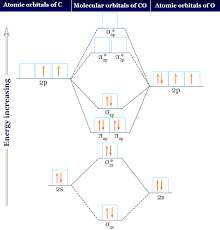
\includegraphics[width=0.6\textwidth]{co_mo.png}
    \caption{Molecular Orbital Diagram for Carbon Monoxide.}
    \label{fig:CO_MO}
\end{figure}
The unique bit is that the $\pi(2p)$ orbitals are lower in energy than the $\sigma(2p)$ orbital. This is also the case for dinitrogen, but not dioxygen. Notice that carbon nitrogen, and oxygen, all lie in the same period of the periodic table, with the ordering from left to right in the same order as they were just presented. Because carbon is further to the left, its valence 2s atomic orbitals will be held further out from the nucleus because of a lack of protons. Because of this, there is significant mixing between the $\sigma (2s)$ and $\sigma(2p)$ orbitals, which pushes the $\sigma(2p)$ orbital higher in energy. 
\subsection{}
(c) When the CO is adsorbed to a transition metal surface, describe the various bonding and antibonding interactions and how they impact the strength of CO binding to transition metals.\\
\subsubsection{Solution}
The highest molecular orbital on carbon monoxide is the sigma 2p, whereas the lowest unoccupied molecular orbital is the pi star 2p; these are the frontier orbitals that will be involved in bonding. The bonding interaction will involve the donation of electron density from the filled sigma 2p orbital into empty d orbitals on the transition metal surface. Then, there is the so-called back-bonding which involves the donation of electron density from filled d orbitals on the transition metal surface into the empty pi star 2p orbital on carbon monoxide.

\subsection{}
(d) How does the bond strength between carbon and oxygen change within a carbon monoxide molecule due to the adsorption of carbon monoxide at a transition metal surface?

\subsubsection{Solution}
It will do so due to the back-bonding phenomenon I mentioned before, which involves the metal d orbital donating to the carbon monoxide pi star orbital; but this pi star orbital is an antibonding orbital from the perspective of carbon monoxide, so it will weaken the carbon-oxygen bond.

\section*{Problem 3. Vanadium Flow Battery Revisited}
In problem set 2, you calculated the open circuit potential of a Vanadium flow battery as a function of concentration:\\
% \includegraphics[max width=\textwidth, center]{2025_10_17_e90f1bdb25229e42e1d0g-3}

$$
\begin{aligned}
V O_{2}^{+}+2 H^{+}+e^{-} & \rightleftarrows V O^{2+}+\mathrm{H}_{2} O \\
V^{2+} & \rightleftarrows V^{3+}+e^{-} \\
\hline V^{2+}+V O_{2}^{+}+2 H^{+} & \rightleftarrows V O^{2+}+V^{3+}+\mathrm{H}_{2} O
\end{aligned}
$$

$$
\begin{gathered}
E_{e q}[V]=E_{e q}^{0}-\frac{R T}{F} \ln \left\{\left(\frac{C_{V O^{2+}}}{C_{V O 2^{+}} \cdot C_{H^{+}}^{2}}\right)\left(\frac{C_{V^{3+}}}{C_{V^{2+}}}\right)\right\} \\
c_{i}(t)=c_{0, i}+\frac{I v_{i}}{F V} t
\end{gathered}
$$

Assume the initial concentrations of $\mathrm{V}^{2+}, \mathrm{V}^{3+}, \mathrm{VO}^{2+}$, and $\mathrm{VO}_{2}{ }^{+}$are $0.1,0.1,1$, and 1 M , respectively, and the pH of the electrolyte is 1 , calculate the actual open circuit potential of the vanadium flow battery.\\
\subsection{}
(a) Assume Butler-Volmer kinetics, charge transfer coefficients of $\frac{1}{2}$, an exchange current density for each electrode equal to $0.5 \mathrm{~A} / \mathrm{m}^{2}$ (a constant independent of concentration), and an electrode area of $1 \mathrm{~m}^{2}$. Plot the potential of the cell during a 1 hour discharge at 1 A as function of time. Note that the full cell potential will be defined as: $E=E_{\text {eq }}+\eta_{\text {cathode }}-\eta_{\text {anode }}$\\
\subsubsection{Solution}
See the notebook.
\subsection{}
(b) You now take your "discharged" cell and charge it back to the initial state described in part a with 1 A of current. What is the overall power efficiency of this cell? Power efficiency is defined as: $P_{\text {efficiency }}=\frac{\int I V_{\text {discharge }} d t}{\int I V_{\text {charge }} d t}$.
\subsubsection{Solution}
To approach this problem, we can analyze the expression given for the power efficiency; we know the current is the same in both directions, so we can simplify the expression to:
\begin{equation}
P_{\text {efficiency }}=\frac{\int V_{\text {discharge }} d t}{\int V_{\text {charge }} d t}
\end{equation}
These quantities can be determined as follows. We can start from the definition of cell voltage as
$$
E_{\text {cell }}=E_{\text {cathode }}-E_{\text {anode }}
$$
so at equilibrium (no current flowing), we have
$$
E_{\text {cell, eq }}=E_{\text {cathode, eq }}-E_{\text {anode, eq }}=E_{\text {eq }}
$$
But we know that in the charging or discharging processes come current is flowing, so the electrodes are not at equilibrium and have an overpotential shift defined as:
\begin{align}
    \eta_{\text {electrode }}&=E_{\text {electrode, actual }}-E_{\text {electrode, eq }}\\
    \implies E_{\text {electrode, actual }}&=E_{\text {electrode, eq }}+\eta_{\text {electrode }}
\end{align}
and substitute this into the full cell equation  gives:
\begin{align}
E_{\text {cell, actual }}&=E_{\text {cathode, actual }}-E_{\text {anode, actual }}\\
&=\left(E_{\text {cathode, eq }}+\eta_{\text {cathode }}\right)-\left(E_{\text {anode, eq }}+\eta_{\text {anode }}\right) \\
&=E_{\text {cathode, eq }}-E_{\text {anode, eq }}+\eta_{\text {cathode }}-\eta_{\text {anode }} \\
&= E_{\text {eq }} + \eta_{\text {cathode }} - \eta_{\text {anode }}
\end{align}
Now, the signs of $\eta_{\text {anode }}$ and $\eta_{\text {cathode }}$ depend on whether you're discharging or charging, so
$$
E_{\text {discharge }}=E_{\text {eq }}-\left(\left|\eta_{\text {anode }}\right|+\left|\eta_{\text {cathode }}\right|\right)
$$
For charge, the signs reverse:
$$
E_{\text {charge }}=E_{\text {eq }}+\left(\left|\eta_{\text {anode }}\right|+\left|\eta_{\text {cathode }}\right|\right)
$$
But in our notebook, we have some functions which are able to determine these quantities, and then we can just numerically integrate over all of the time steps. This gives a power efficiency of $\approx 86 \%$.

\end{document}